\graphicspath{{../giaitoancungbi/robin/}}
\begingroup
\AddToShipoutPicture*{\put(65,600){
\includegraphics[scale=0.75]{../robin/tieude1.pdf}}} % %Image background
\centering
\endgroup
\vspace*{35pt}
\definecolor{abc}{cmyk}{0,0.85,0.7,0}

\textbf{Robin là một chú ếch tinh nghịch. Chú luôn thích đi du lịch, khám phá các vùng đất mới.~Các bé hãy cùng Bi giải đáp các câu hỏi nảy sinh trong những cuộc phiêu lưu của Robin nhé!}

\vspace*{5pt}

	\textbf{\textit{Câu hỏi $\pmb{1.}$}} {\color{abc}\textbf{Trong một chuyến phiêu lưu,  Robin dừng chân khám phá đảo “Xoắn ốc”. Ngay khi Robin vừa đặt chân lên đảo, có một hàng rào kỳ lạ hình xoắn ốc bỗng dựng lên, như ở Hình $1$, nhốt chú bên trong hàng rào (trong hình, hàng rào được thể hiện bởi đường màu đen). Trên đảo có hai khóm cây hoa, $\pmb 
	A$ và $\pmb B$. Đố Bi và các bé biết, có khóm cây hoa nào nằm trong hàng rào hay không? Nếu có thì là khóm cây nào, $\pmb A$ hay $\pmb B$, hay cả $\pmb A$ và $\pmb B$? Vì sao?}}
	\begin{figure}[H]
		\centering
		\vspace*{-5pt}
		\captionsetup{labelformat= empty, justification=centering}
		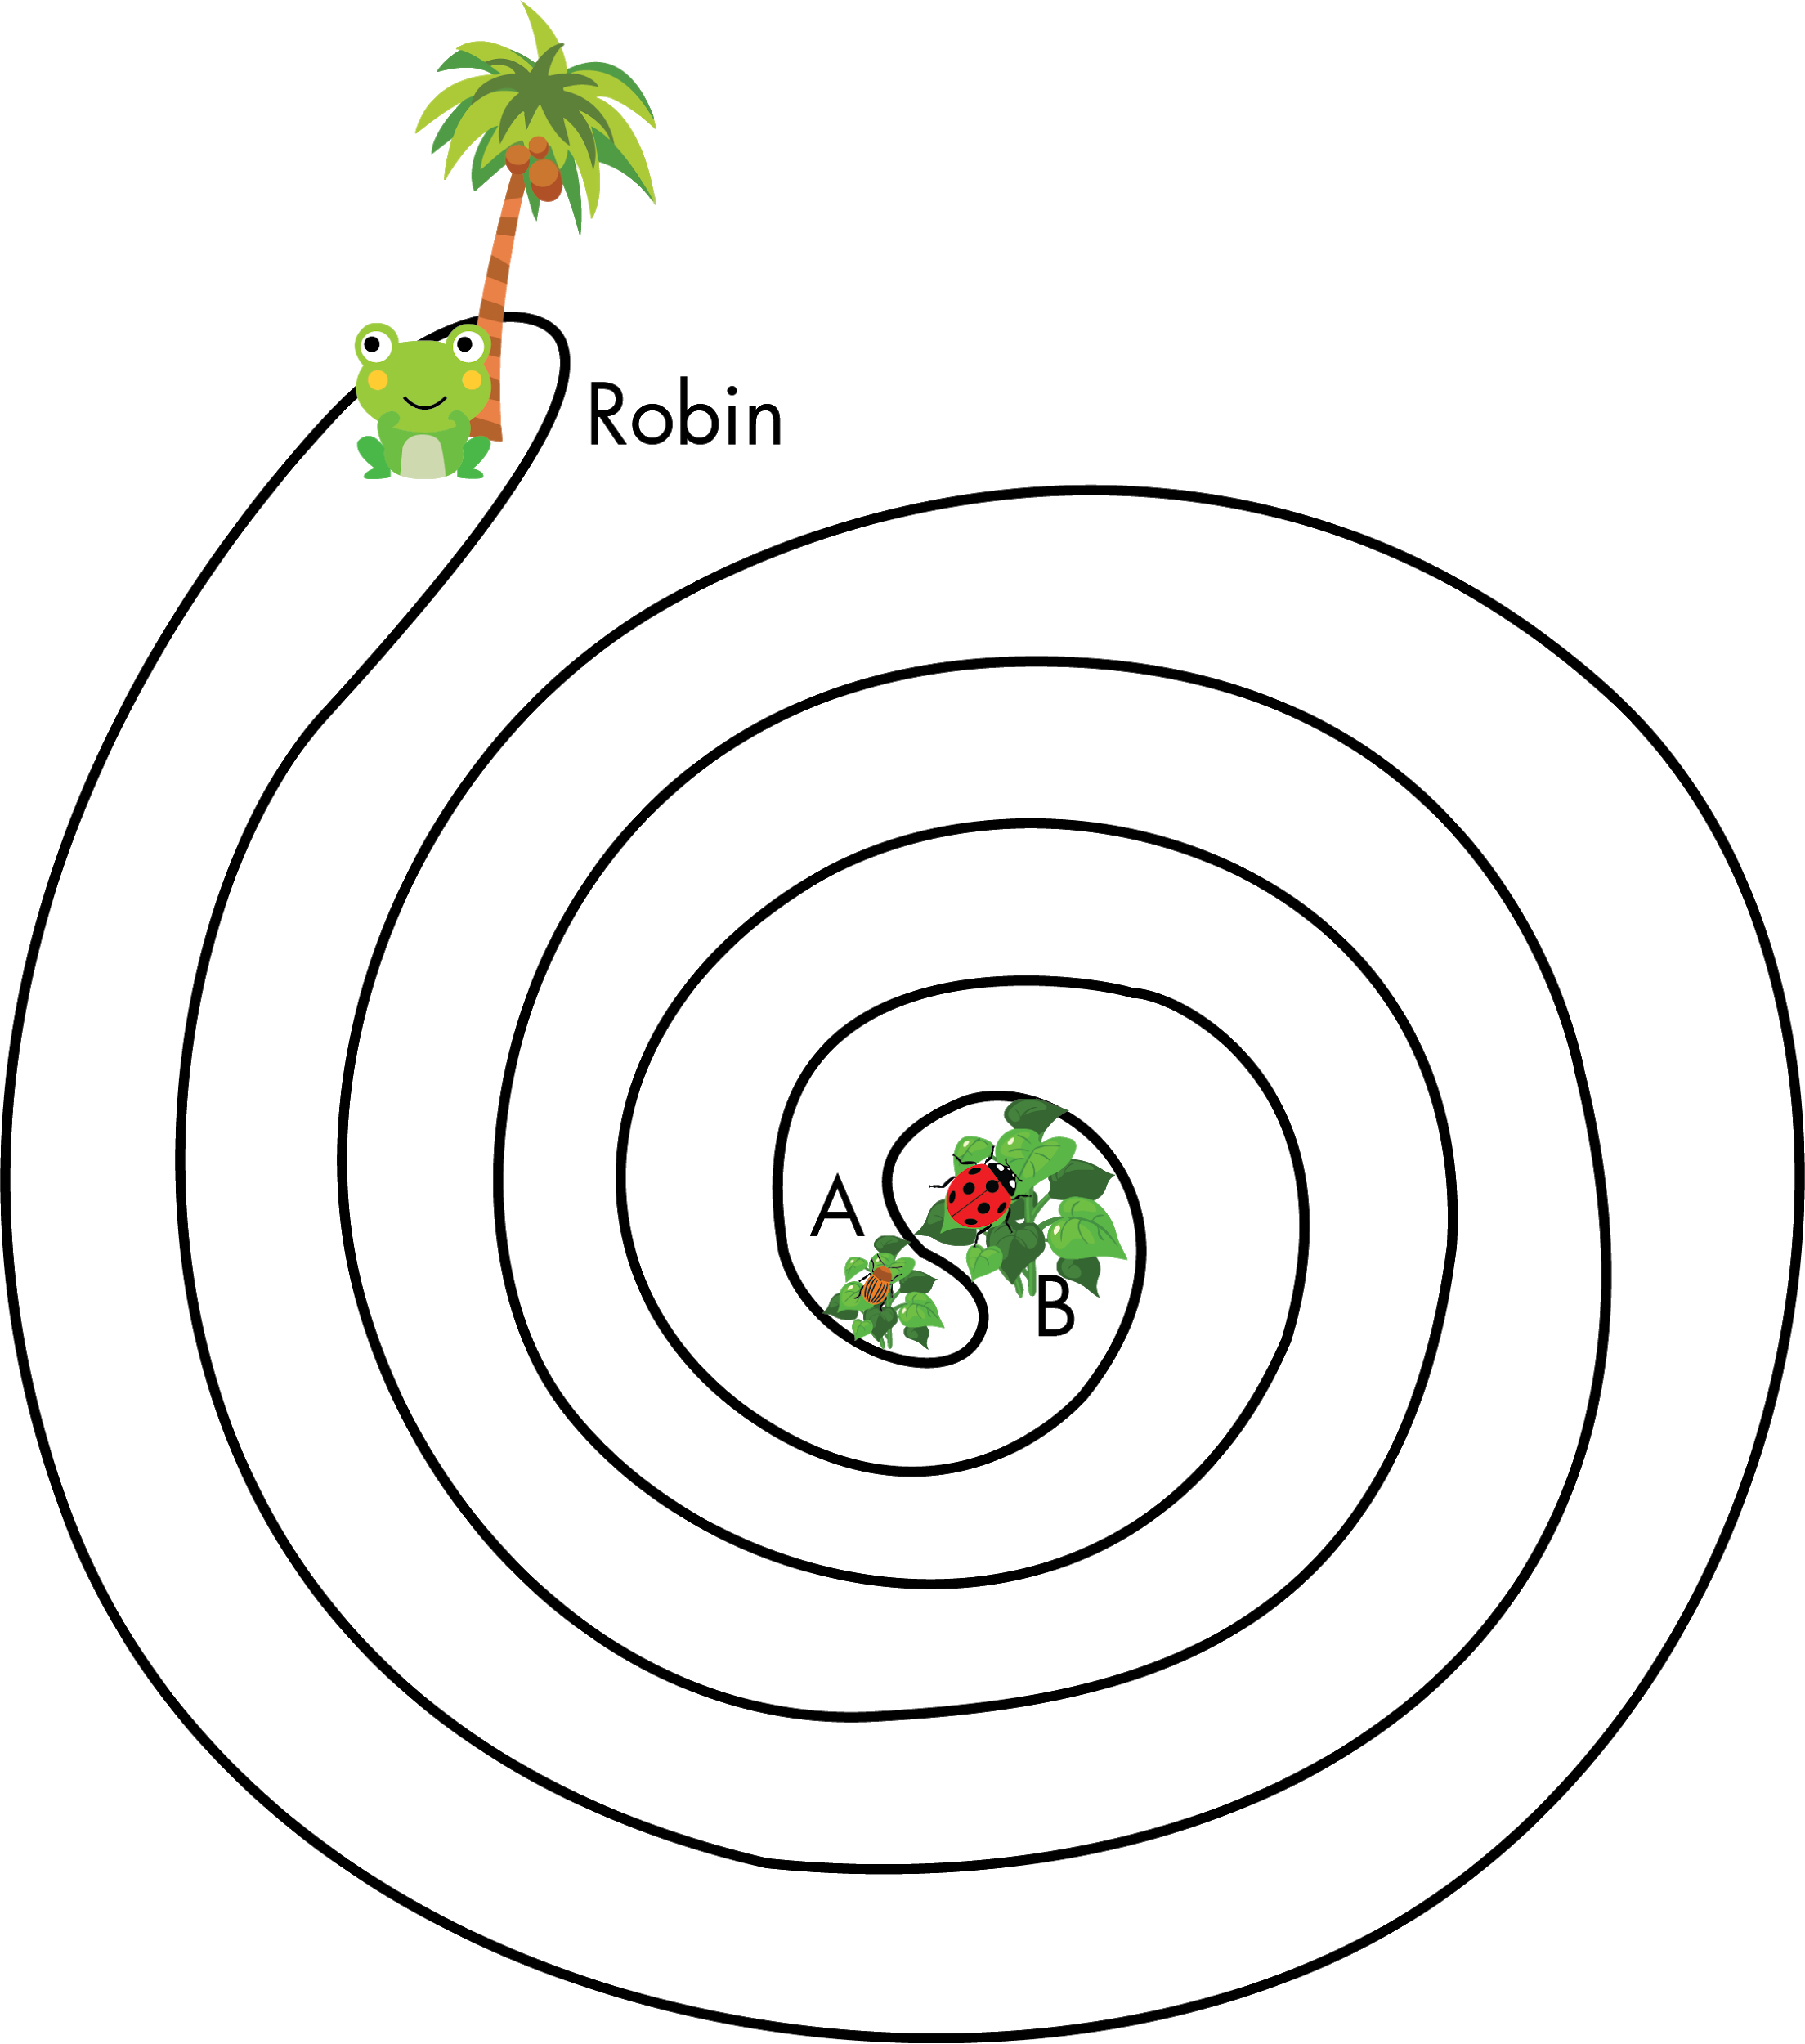
\includegraphics[width=0.38\textwidth]{1}
		\caption{\small\textit{Hình $1.$}}
		\vspace*{-10pt}
	\end{figure}
	Chúng mình cùng Bi suy luận nha.
	\vskip 0.1cm
	Để biết có khóm cây hoa nào chịu cùng cảnh ngộ nằm trong hàng rào như Robin hay không, chúng mình cần phân biệt được hai phần đảo, phần nằm trong và phần nằm ngoài hàng rào. Điều này hẳn ai cũng biết, vấn đề chỉ là làm thế nào để phân biệt được, khi hàng rào xoắn tít như mê cung thế kia.
	\vskip 0.1cm
	Chắc bé, cũng như Bi, đã từng nhiều lần nhìn thấy, nhiều lần xem các bản đồ (bản đồ Việt Nam, bản đồ thế giới,\ldots). Và hẳn cũng như Bi, bé thấy bản đồ nào cũng được tô bởi nhiều màu sắc khác nhau, phải không nào? Sao lại thế~nhỉ?
	\vskip 0.1cm
	Quan sát kỹ các tấm bản đồ, hẳn bé, cũng như Bi, sẽ phát hiện ra rằng, tấm bản đồ được tô bởi nhiều màu sắc khác nhau nhằm giúp người xem phân biệt được đất liền với đại dương, biển cả, phân biệt được lãnh thổ của quốc gia này với lãnh thổ của quốc gia khác, phân biệt được lãnh thổ của tỉnh này với lãnh thổ của tỉnh khác, \ldots. Nhờ phát hiện này mà Bi đã nảy ra sáng kiến dùng màu sắc để phân biệt phần đảo nằm trong hàng rào với phần đảo nằm ngoài hàng rào đấy.
	\vskip 0.1cm
	Vì đường viền đen là ranh giới giữa phần đảo nằm trong và nằm ngoài hàng rào, và do chú ếch Robin nằm trong hàng rào, nên để tô được phần đảo nằm trong hàng rào, Bi đã đặt bút màu vào nơi có chú ếch Robin trong Hình $1$, rồi tô màu sao cho trong quá trình tô, bút màu không rê qua đường viền đen ở bất cứ chỗ nào. Bằng cách đó, từ Hình $1$, Bi đã thu được Hình $2$, mà ở đó, phần được tô màu chính là phần đảo nằm trong hàng rào.
	\begin{figure}[H]
		\centering
		%\vspace*{-5pt}
		\captionsetup{labelformat= empty, justification=centering}
		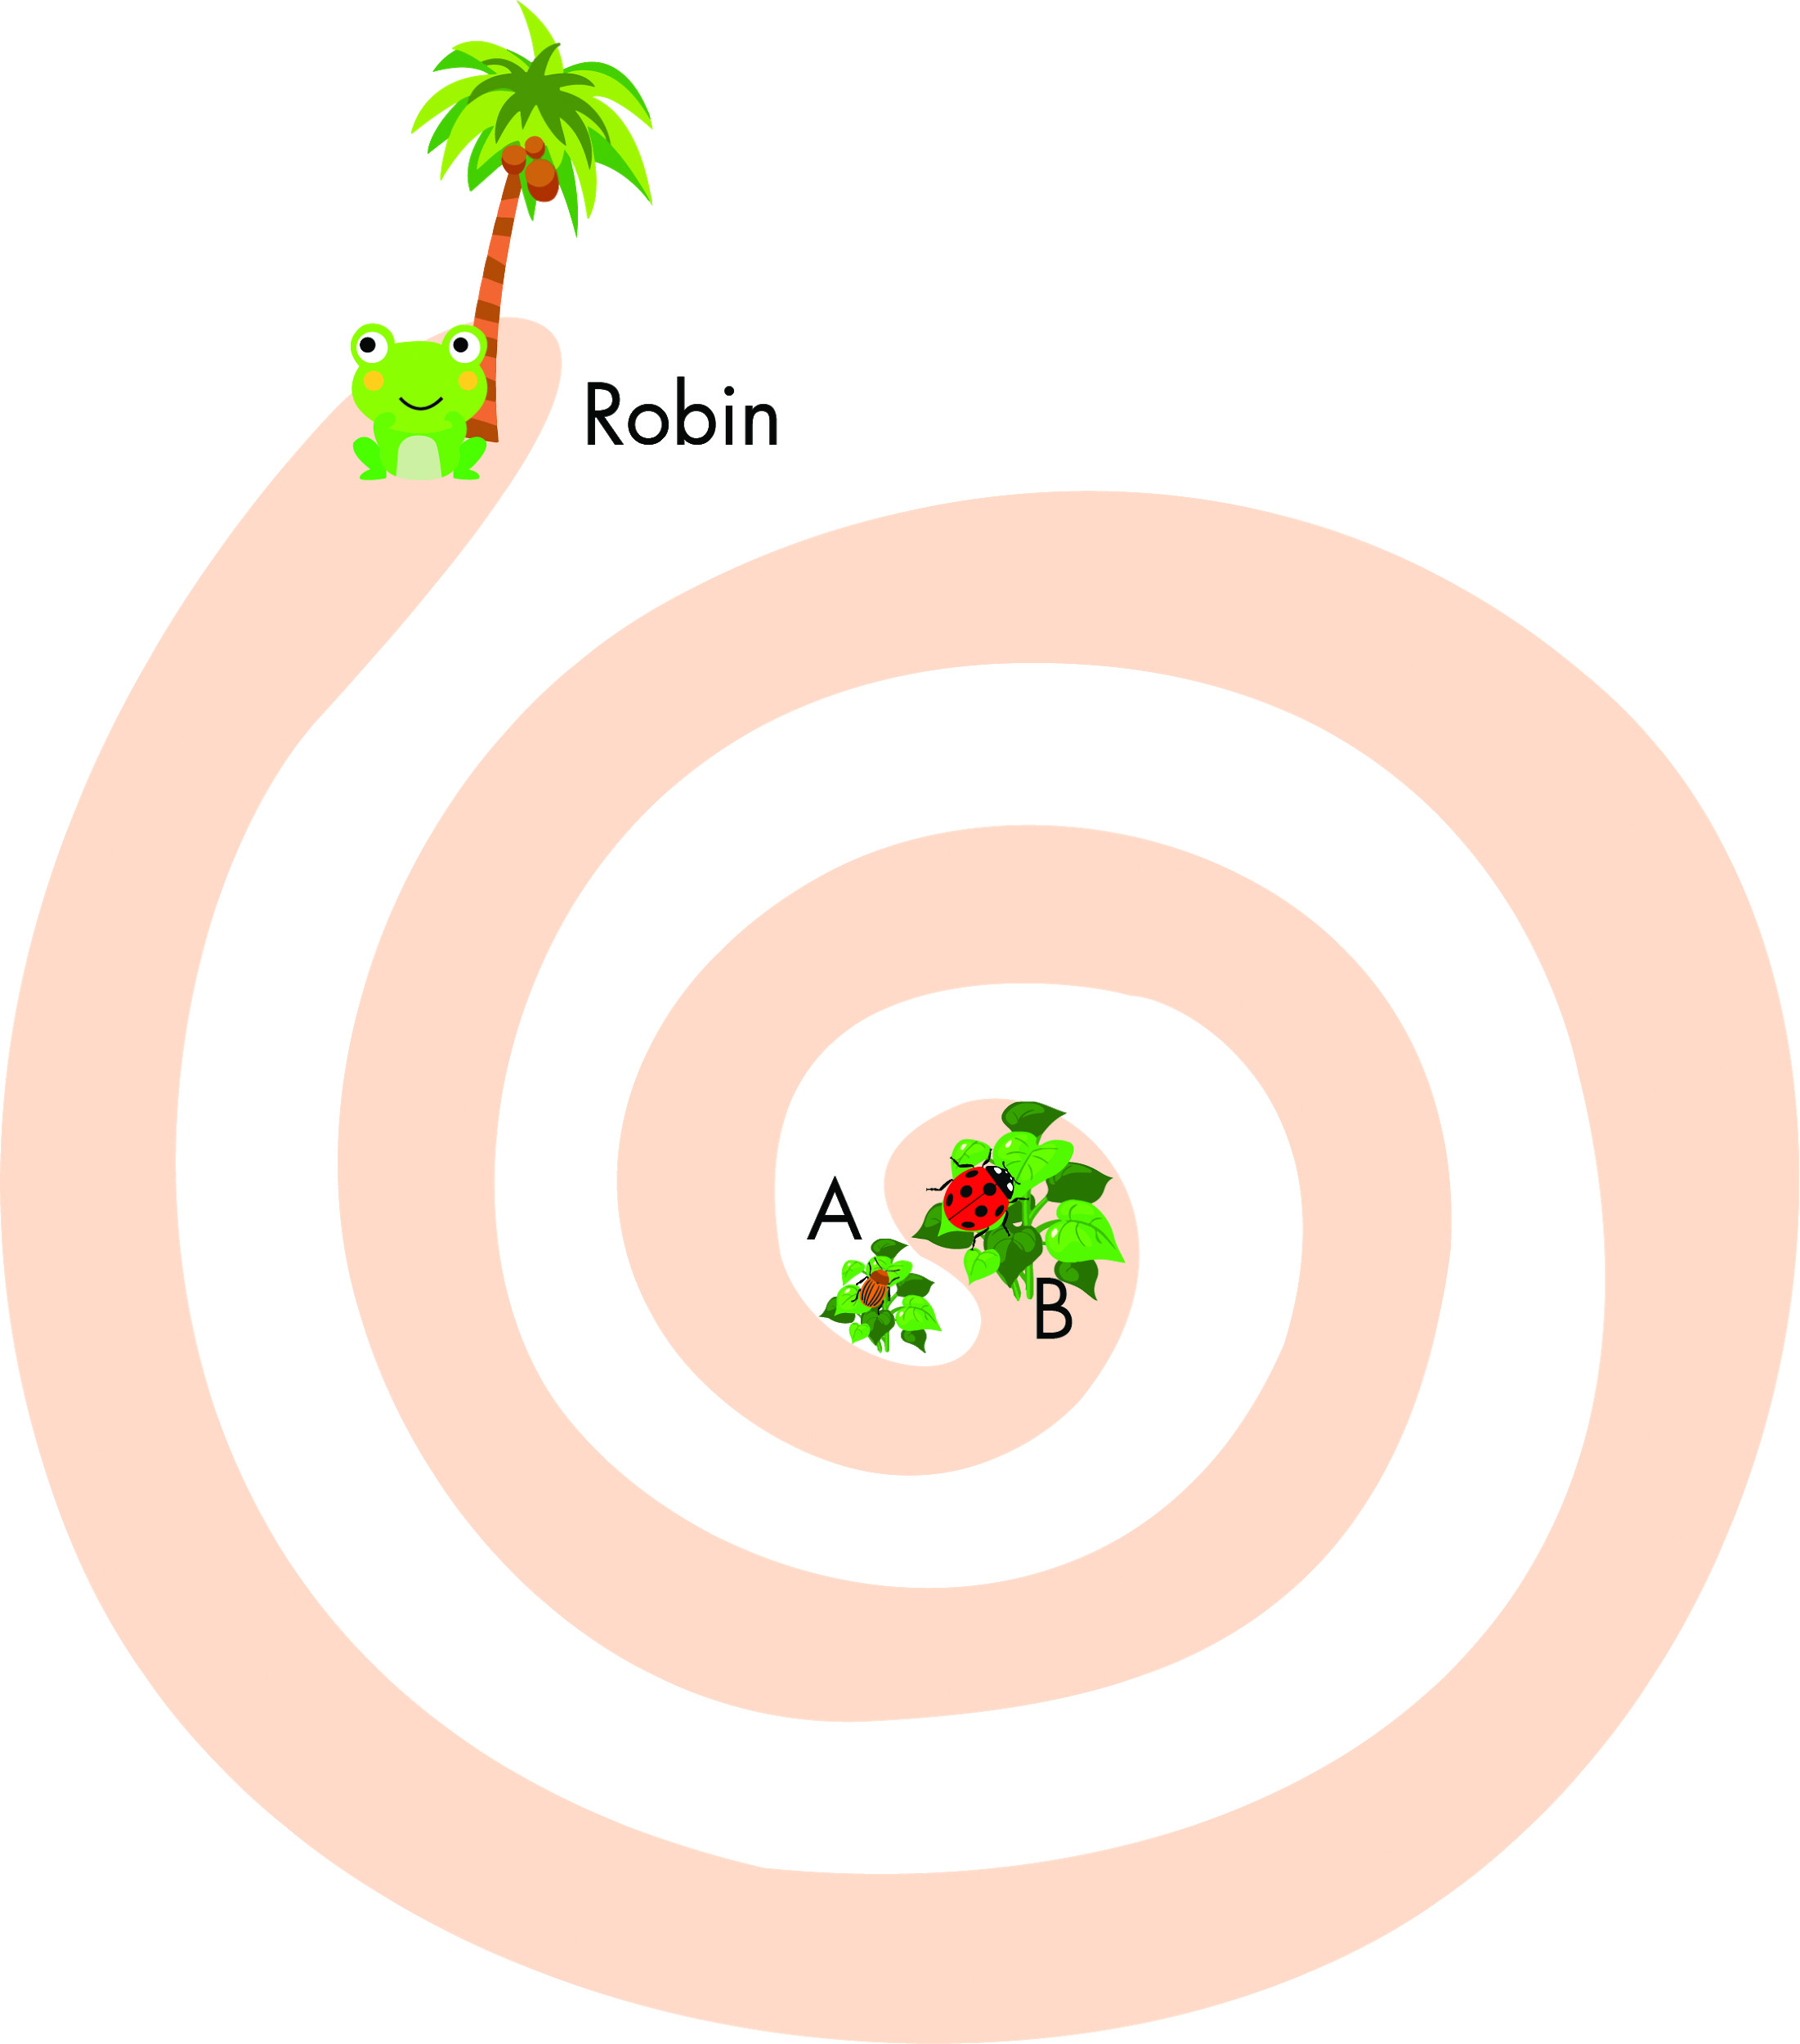
\includegraphics[width=0.35\textwidth]{2}
		\caption{\small\textit{Hình 2}}
		\vspace*{-15pt}
	\end{figure}
 	Thế là, nhờ sáng kiến tô màu của Bi, chúng  mình đã trả lời được câu hỏi $1$: Trong hai khóm cây hoa, $A$ và $B$, chỉ có khóm $B$ nằm trong hàng rào.
	\vskip 0.1cm
	\textbf{\textit{Câu hỏi $\pmb{2.}$} {\color{abc}Trong một cuộc phiêu lưu khác, chú ếch Robin đã dừng chân trên một hòn đảo có hình thù rất kỳ lạ, được mô tả ở Hình $3$ (trong hình, đường màu đen thể hiện ranh giới giữa đảo và biển). Chú thấy trong vùng đảo có chín con cá sấu (xem Hình $3$); trong đó, có những con nằm trên bờ và có cả những con đang ở dưới nước. Đố Bi và các bé biết, trong Hình $3$, có bao nhiêu con cá sấu nằm trên bờ?}}
	\begin{figure}[H]
		\centering
		\vspace*{-10pt}
		\captionsetup{labelformat= empty, justification=centering}
		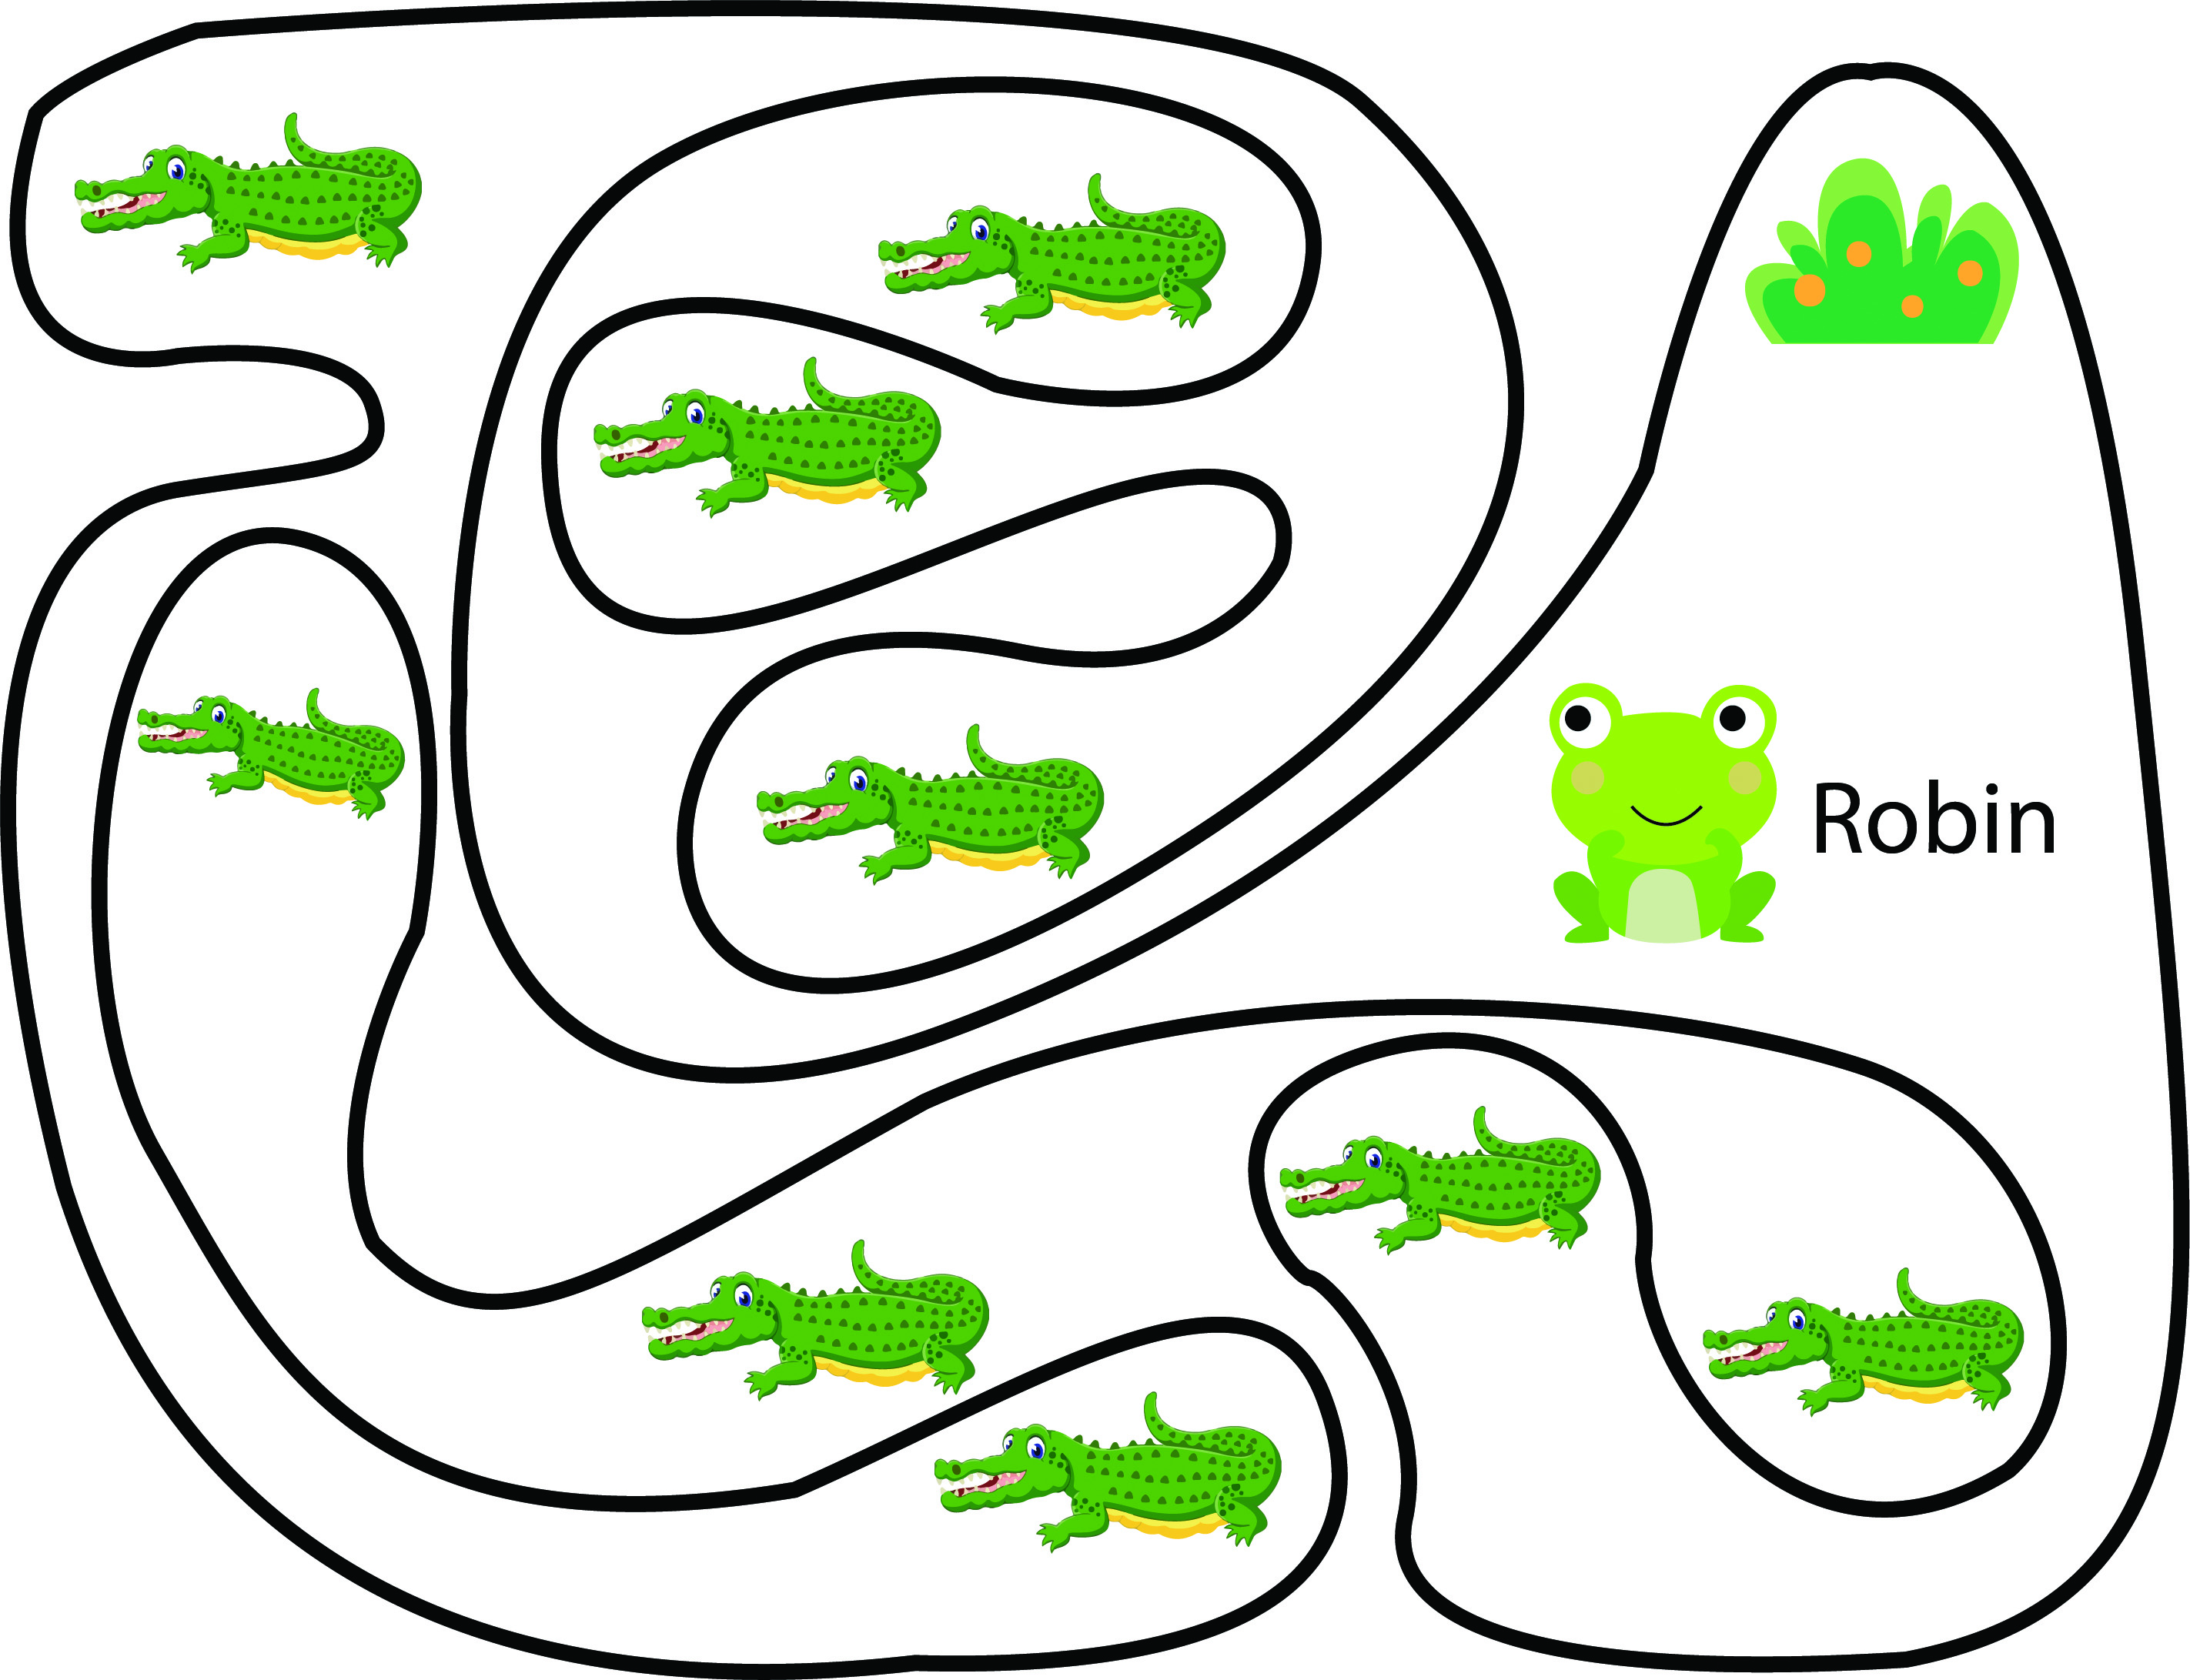
\includegraphics[width=0.45\textwidth]{pic12}
%		\vspace*{-5pt}
		\caption{\small\textit{Hình $3.$}}
		\vspace*{-10pt}
	\end{figure}
	Giải đáp được câu hỏi $1$ rồi thì việc tìm ra câu trả lời cho câu hỏi $2$ không còn chút khó khăn nào nữa, phải không các bé?
	\vskip 0.1cm
	Để biết được có bao nhiêu con cá sấu nằm trên bờ, chúng mình cần phân biệt được phần đảo và phần biển. Bằng cách tô màu tương tự trên, từ Hình $3$, Bi đã thu được Hình $4$, mà ở đó, phần được tô màu là phần đảo và phần không có màu là phần biển.
	\begin{figure}[H]
		\centering
		\vspace*{-10pt}
		\captionsetup{labelformat= empty, justification=centering}
		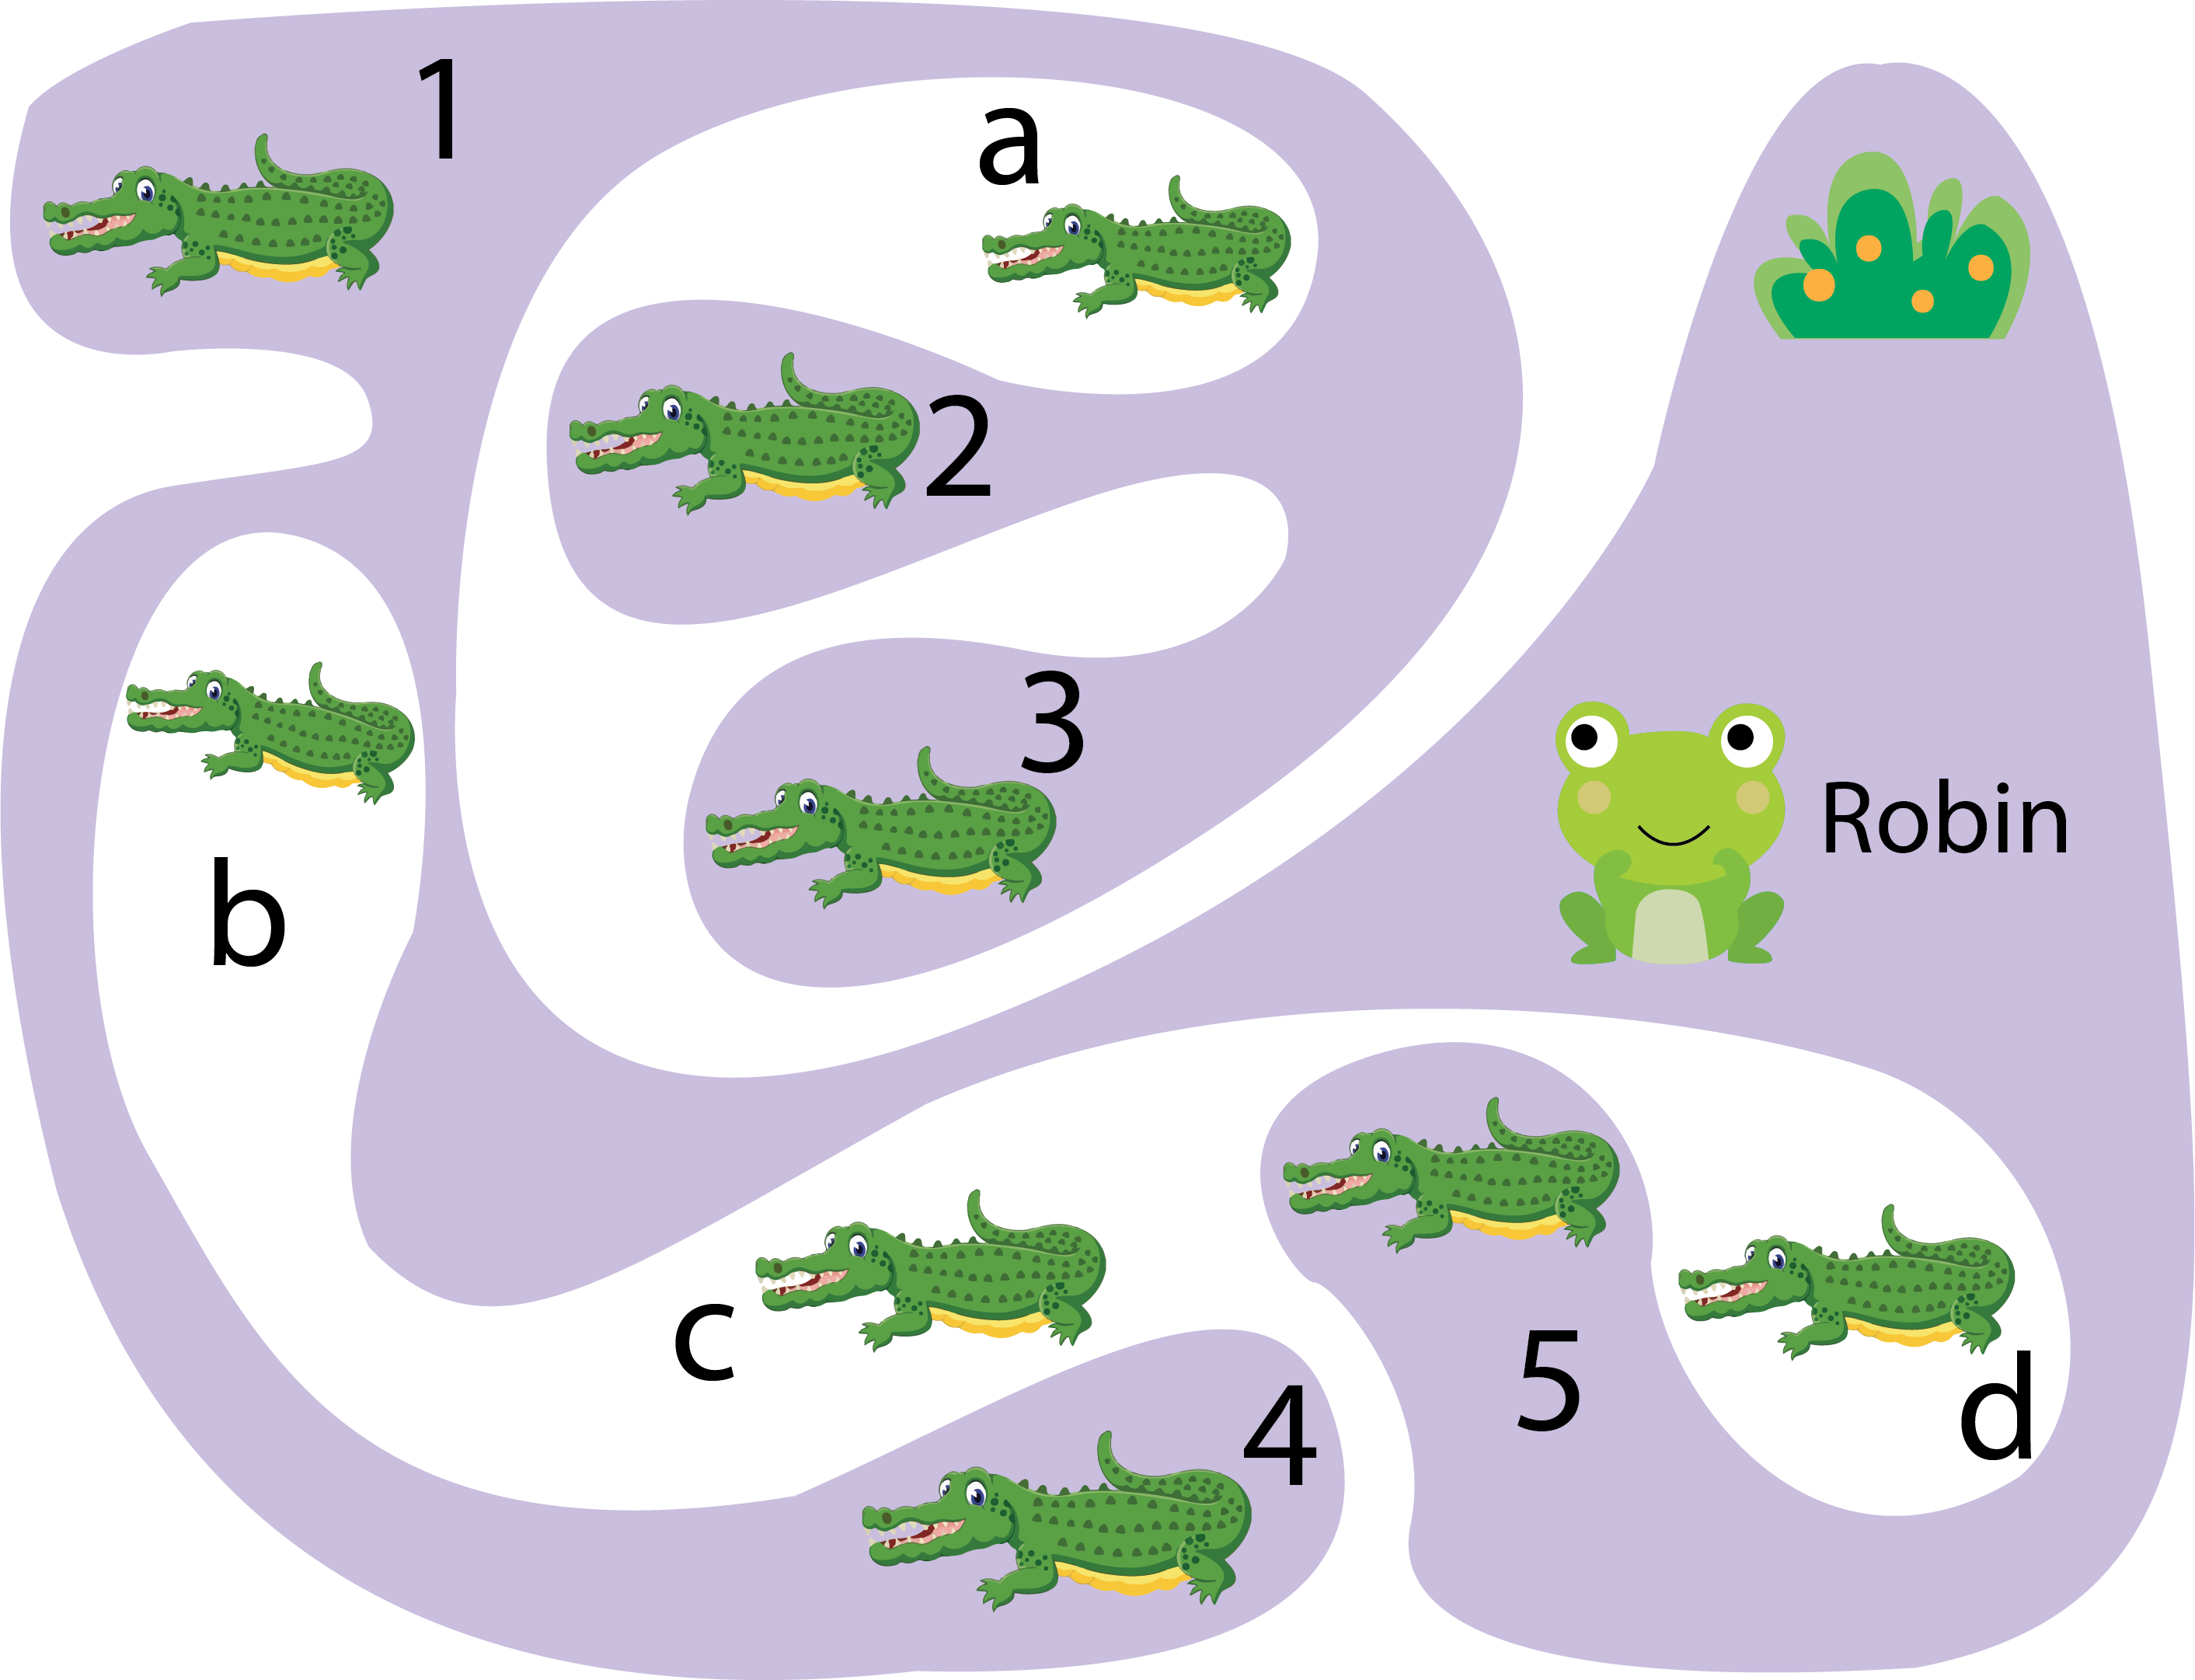
\includegraphics[width=0.45\textwidth]{pic13}
%		\vspace*{-5pt}
		\caption{\small\textit{Hình $4.$}}
		\vspace*{-10pt}
	\end{figure}
	Nhìn Hình $4$, chúng mình đếm được năm con cá sấu nằm trên bờ. Thật đơn giản, các bé nhỉ?
	\vskip 0.1cm
	\textbf{\textit{Câu hỏi $\pmb{3.}$} {\color{abc}Lần này, rất không may, Robin tới một hòn đảo vào đúng lúc đang có một luồng khí nóng và một luồng khí lạnh đang uốn lượn, chuẩn bị đổ bộ vào đảo. Trong  Hình $5$, phần nằm trong đường màu đỏ là phần đảo sẽ chịu ảnh hưởng của luồng khí nóng, và phần nằm trong đường màu xanh là phần đảo sẽ chịu ảnh hưởng của luồng khí lạnh. Ở nơi chịu ảnh hưởng của cả hai luồng khí, sẽ có những cơn lốc xoáy kinh hoàng. Biết rằng, điểm $\pmb A$ nằm ở phần đảo sẽ chịu ảnh hưởng của luồng khí nóng, và điểm $\pmb B$ nằm ở phần đảo sẽ chịu ảnh hưởng của luồng khí lạnh. Đố Bi và các bé biết, nếu Robin, từ vị trí đang đứng của mình, chỉ có thể di}}
	\begin{figure}
		\vspace*{-5pt}
		\centering
		\captionsetup{labelformat=empty, justification=centering}
		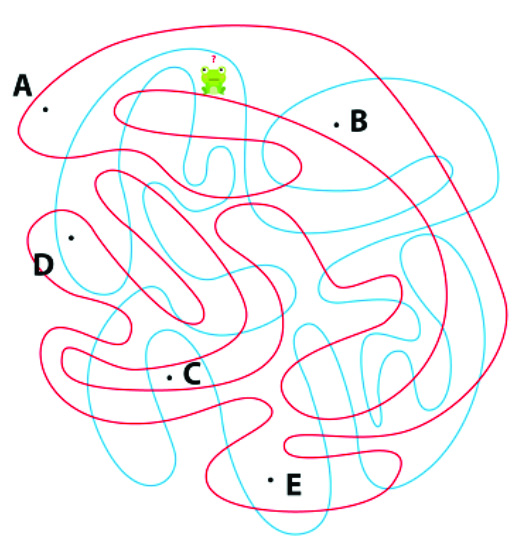
\includegraphics[scale=0.38]{5}
		\caption{\textit{\small Hình $5.$}}
		\vspace*{-15pt}
	\end{figure}
	\textbf{{\color{abc}chuyển đến các điểm~$\pmb C$, $\pmb D$, $\pmb E$ thì chú cần di chuyển đến điểm nào (trong ba điểm đó) để không bị rơi vào vùng có  lốc xoáy?}}
	\vskip 0.1cm
	Rõ ràng, để trả lời được câu hỏi $3$, chúng mình cần phân biệt được ba vùng: phần đảo chịu ảnh hưởng của luồng khí nóng, phần đảo chịu ảnh hưởng của luồng khí lạnh, và phần đảo không chịu ảnh hưởng của luồng khí nào.
	\vskip 0.1cm
	Ở trên, để phân biệt được hai vùng với nhau, chúng mình cần dùng một màu để tô. Vậy, để phân biệt được ba vùng với nhau, chúng mình cần dùng mấy màu để tô, các bé nhỉ? Đúng rồi, các bé nghĩ đúng rồi đấy, hai màu! Để tô được phần đảo chịu ảnh hưởng của luồng khí nóng, chúng mình cần đặt bút màu vào đâu để bắt đầu tô nhỉ? Và để tô được phần đảo chịu ảnh hưởng của luồng khí lạnh, chúng mình cần đặt bút màu vào đâu để bắt đầu tô? Vì điểm $A$ nằm ở phần đảo sẽ chịu ảnh hưởng của luồng khí nóng nên để tô phần đảo này, khi bắt đầu tô, chúng  mình cần đặt bút màu vào nơi có điểm $A$. Tương tự như thế, vì điểm $B$ nằm ở phần đảo sẽ chịu ảnh hưởng của luồng khí lạnh nên để tô phần đảo này, chúng mình cần đặt bút màu vào nơi có điểm $B$ để bắt đầu tô. Các bé có đồng ý  thế không?
	\vskip 0.05cm
	Bi đã dùng màu hồng để tô phần đảo sẽ chịu ảnh hưởng của luồng khí nóng, và dùng màu xanh da trời để tô phần đảo sẽ chịu ảnh hưởng của luồng khí lạnh. Với việc dùng màu như thế, từ Hình $5$, Bi đã thu được Hình $6$ dưới đây.
	\vskip 0.1cm
	\begin{wrapfigure}{r}[0pt]{0.6\linewidth}
		\centering
		\vspace*{-5pt}
		\captionsetup{labelformat=empty, justification=centering}
		
\includegraphics[scale=0.35]{6}
		\vspace*{-10pt}
		\caption{\textit{\small Hình $6.$}}
		\vspace*{-10pt}
	\end{wrapfigure}
	Nhìn Hình $6$, chúng mình ai cũng thấy, các điểm $D$ và $E$ nằm ở vùng sẽ có lốc xoáy, còn điểm $C$ nằm ở vùng an toàn, không chịu ảnh hưởng của bất cứ luồng khí nào. Vì thế, để tránh lốc xoáy, Robin cần khẩn trương di chuyển ngay đến điểm $C$.
	\vskip 0.05cm
	Bây giờ, các bé hãy tự mình suy nghĩ và giải đáp các câu hỏi sau nhé.
	\vskip 0.1cm
	\textbf{\textit{Câu hỏi $\pmb{4.}$} {\color{abc}Trong Hình $7$ có $11$ chú ếch và một cái ao, trên mặt ao có một khóm sen. Đố bé biết có bao nhiêu chú ếch đang ở trên bờ và bao nhiêu chú ếch đang ở dưới ao?}}
	\begin{figure}[H]
		\centering
		\vspace*{-5pt}
		\captionsetup{labelformat= empty, justification=centering}
		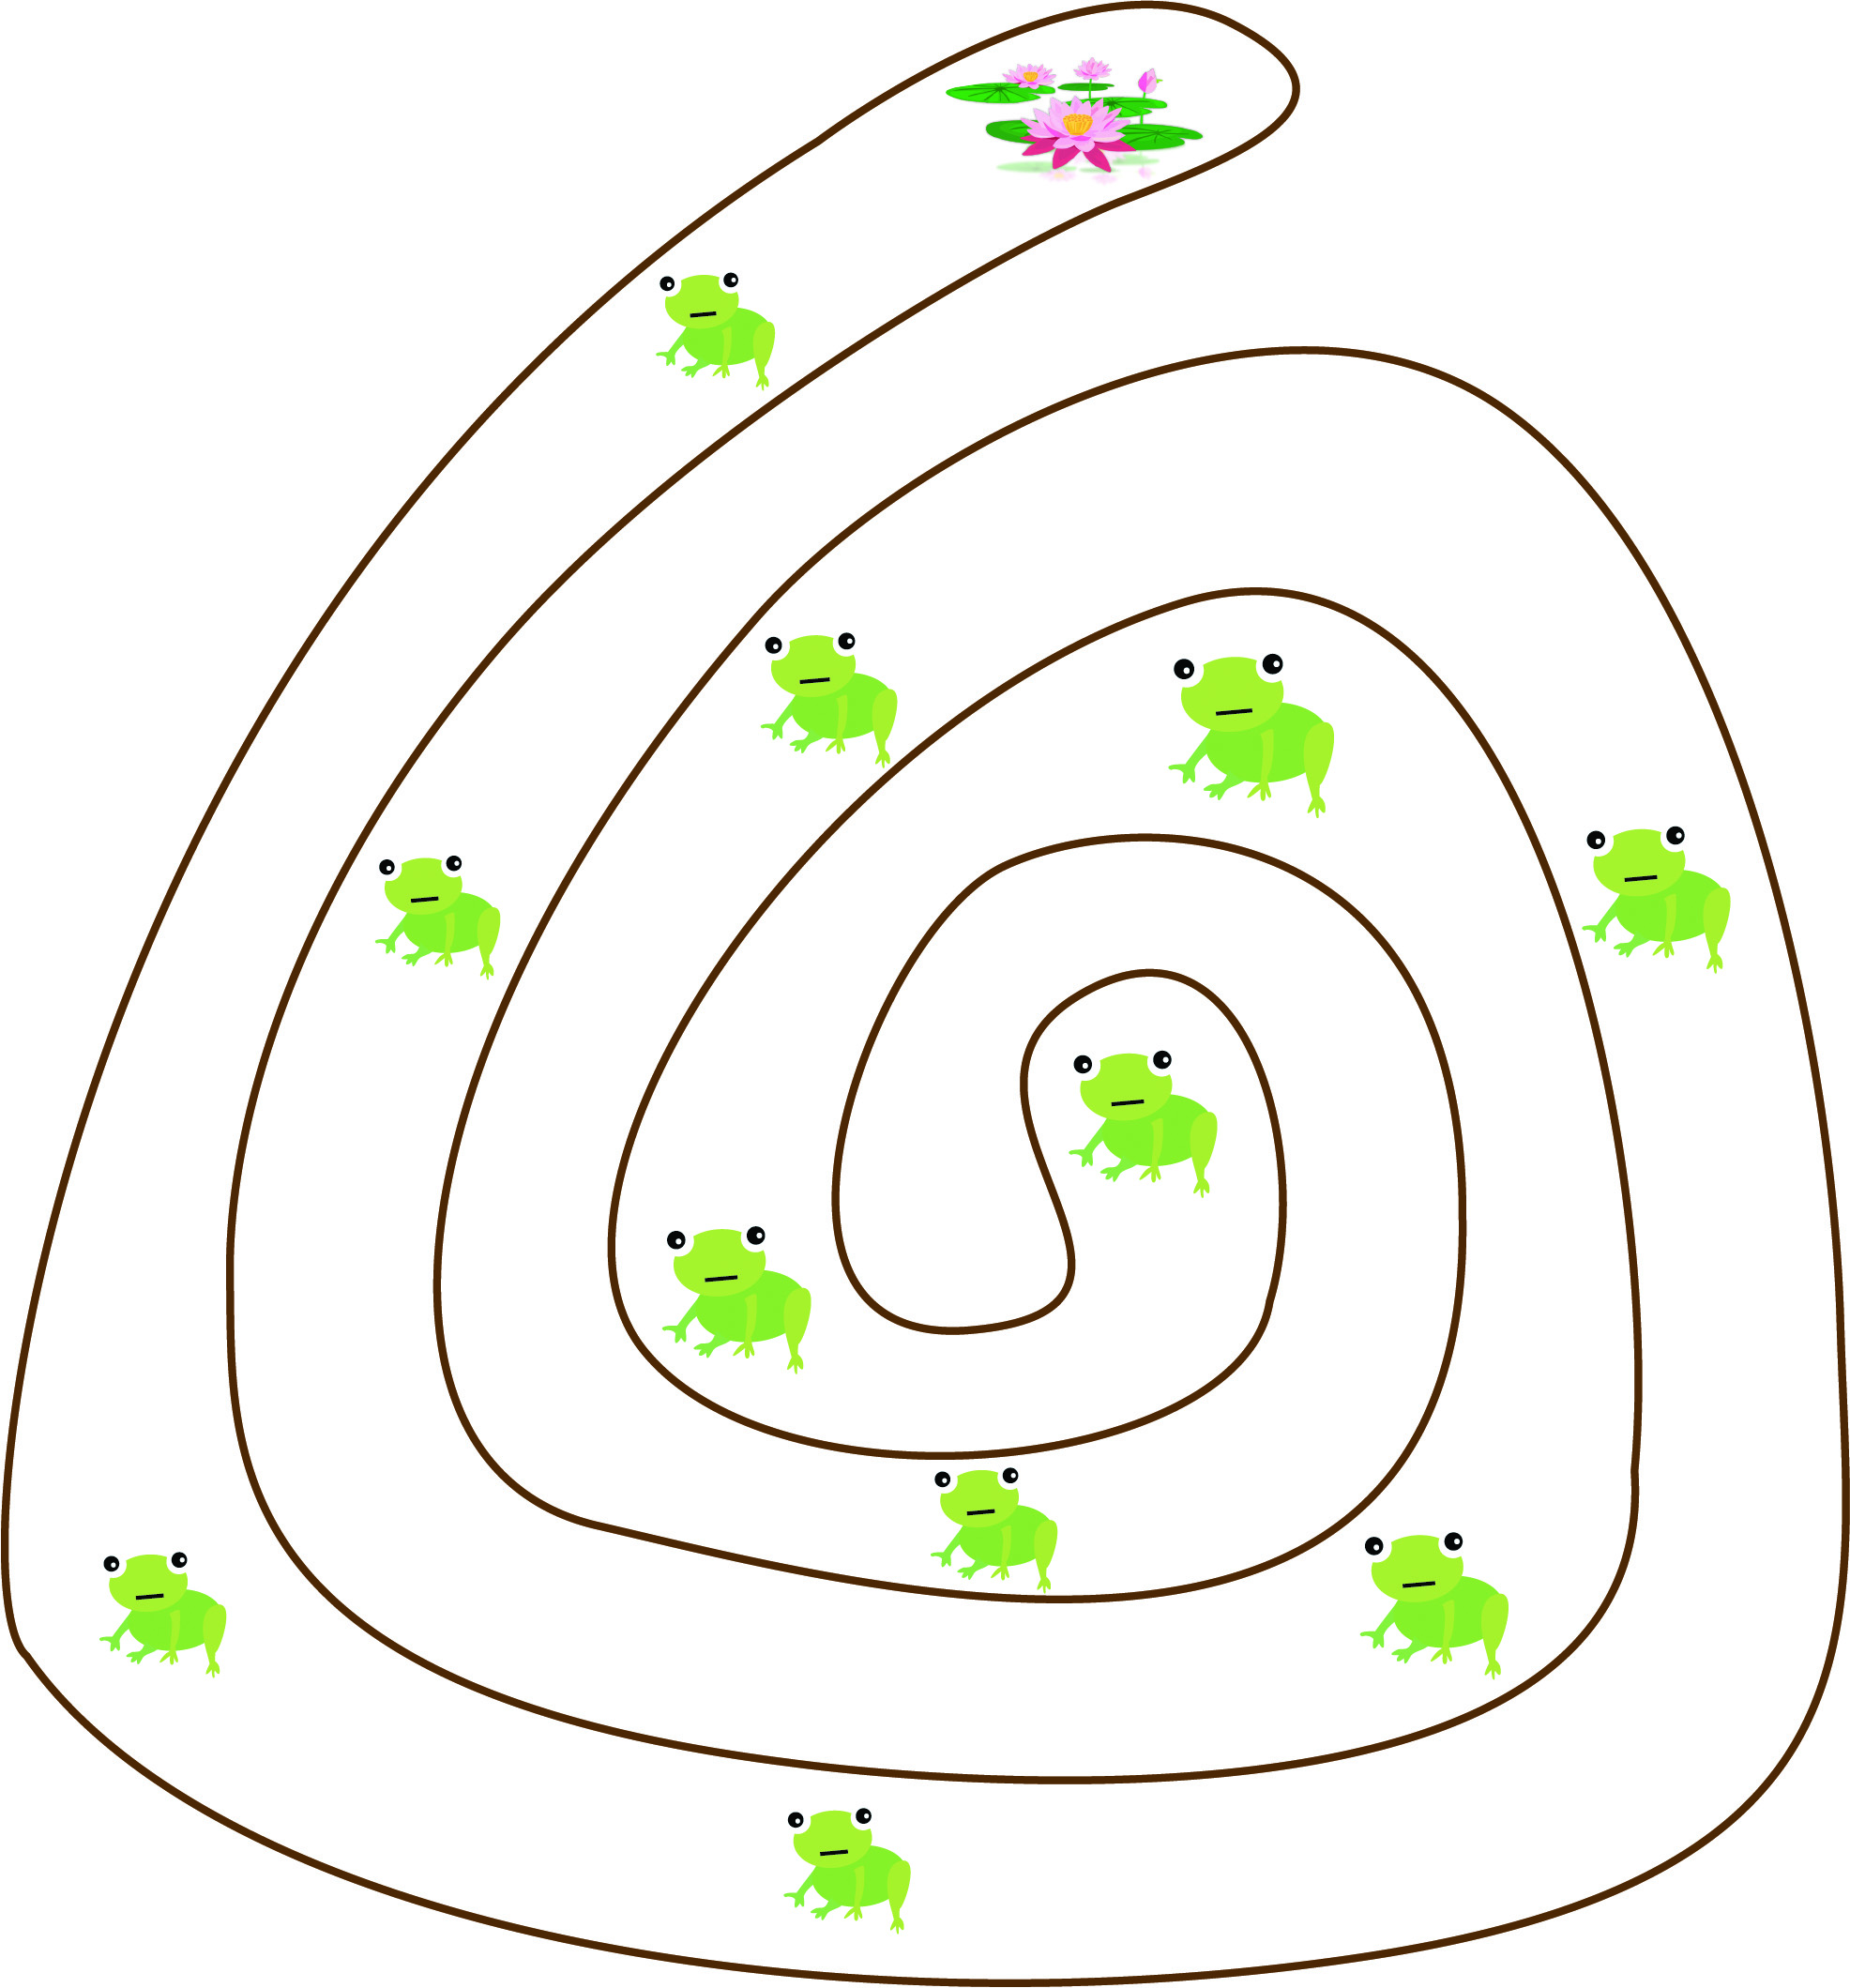
\includegraphics[width=0.4\textwidth]{pic11}
		\caption{\small\textit{Hình $7.$}}
		\vspace*{-10pt}
	\end{figure}
	\textbf{\textit{Câu hỏi $\pmb{5.}$} {\color{abc}Trên một tờ giấy, có một vòng dây màu cam và một vòng dây màu xanh lá cây, như ở Hình $8$. Robin tung $10$ viên kẹo hình trái tim màu đỏ và $10$ viên kẹo hình ngôi sao màu xanh lên trên tờ giấy đó; các viên kẹo rơi xuống tờ giấy như ở Hình $8$. Bé được lấy những viên kẹo màu đỏ chỉ nằm trong vòng dây màu cam và Bi được lấy những viên kẹo màu xanh chỉ nằm trong vòng dây màu  xanh lá cây. Hỏi bé và Bi, ai lấy được nhiều kẹo hơn? Vì sao?}}
	\begin{figure}[H]
		\centering
		\vspace*{-5pt}
		\captionsetup{labelformat= empty, justification=centering}
		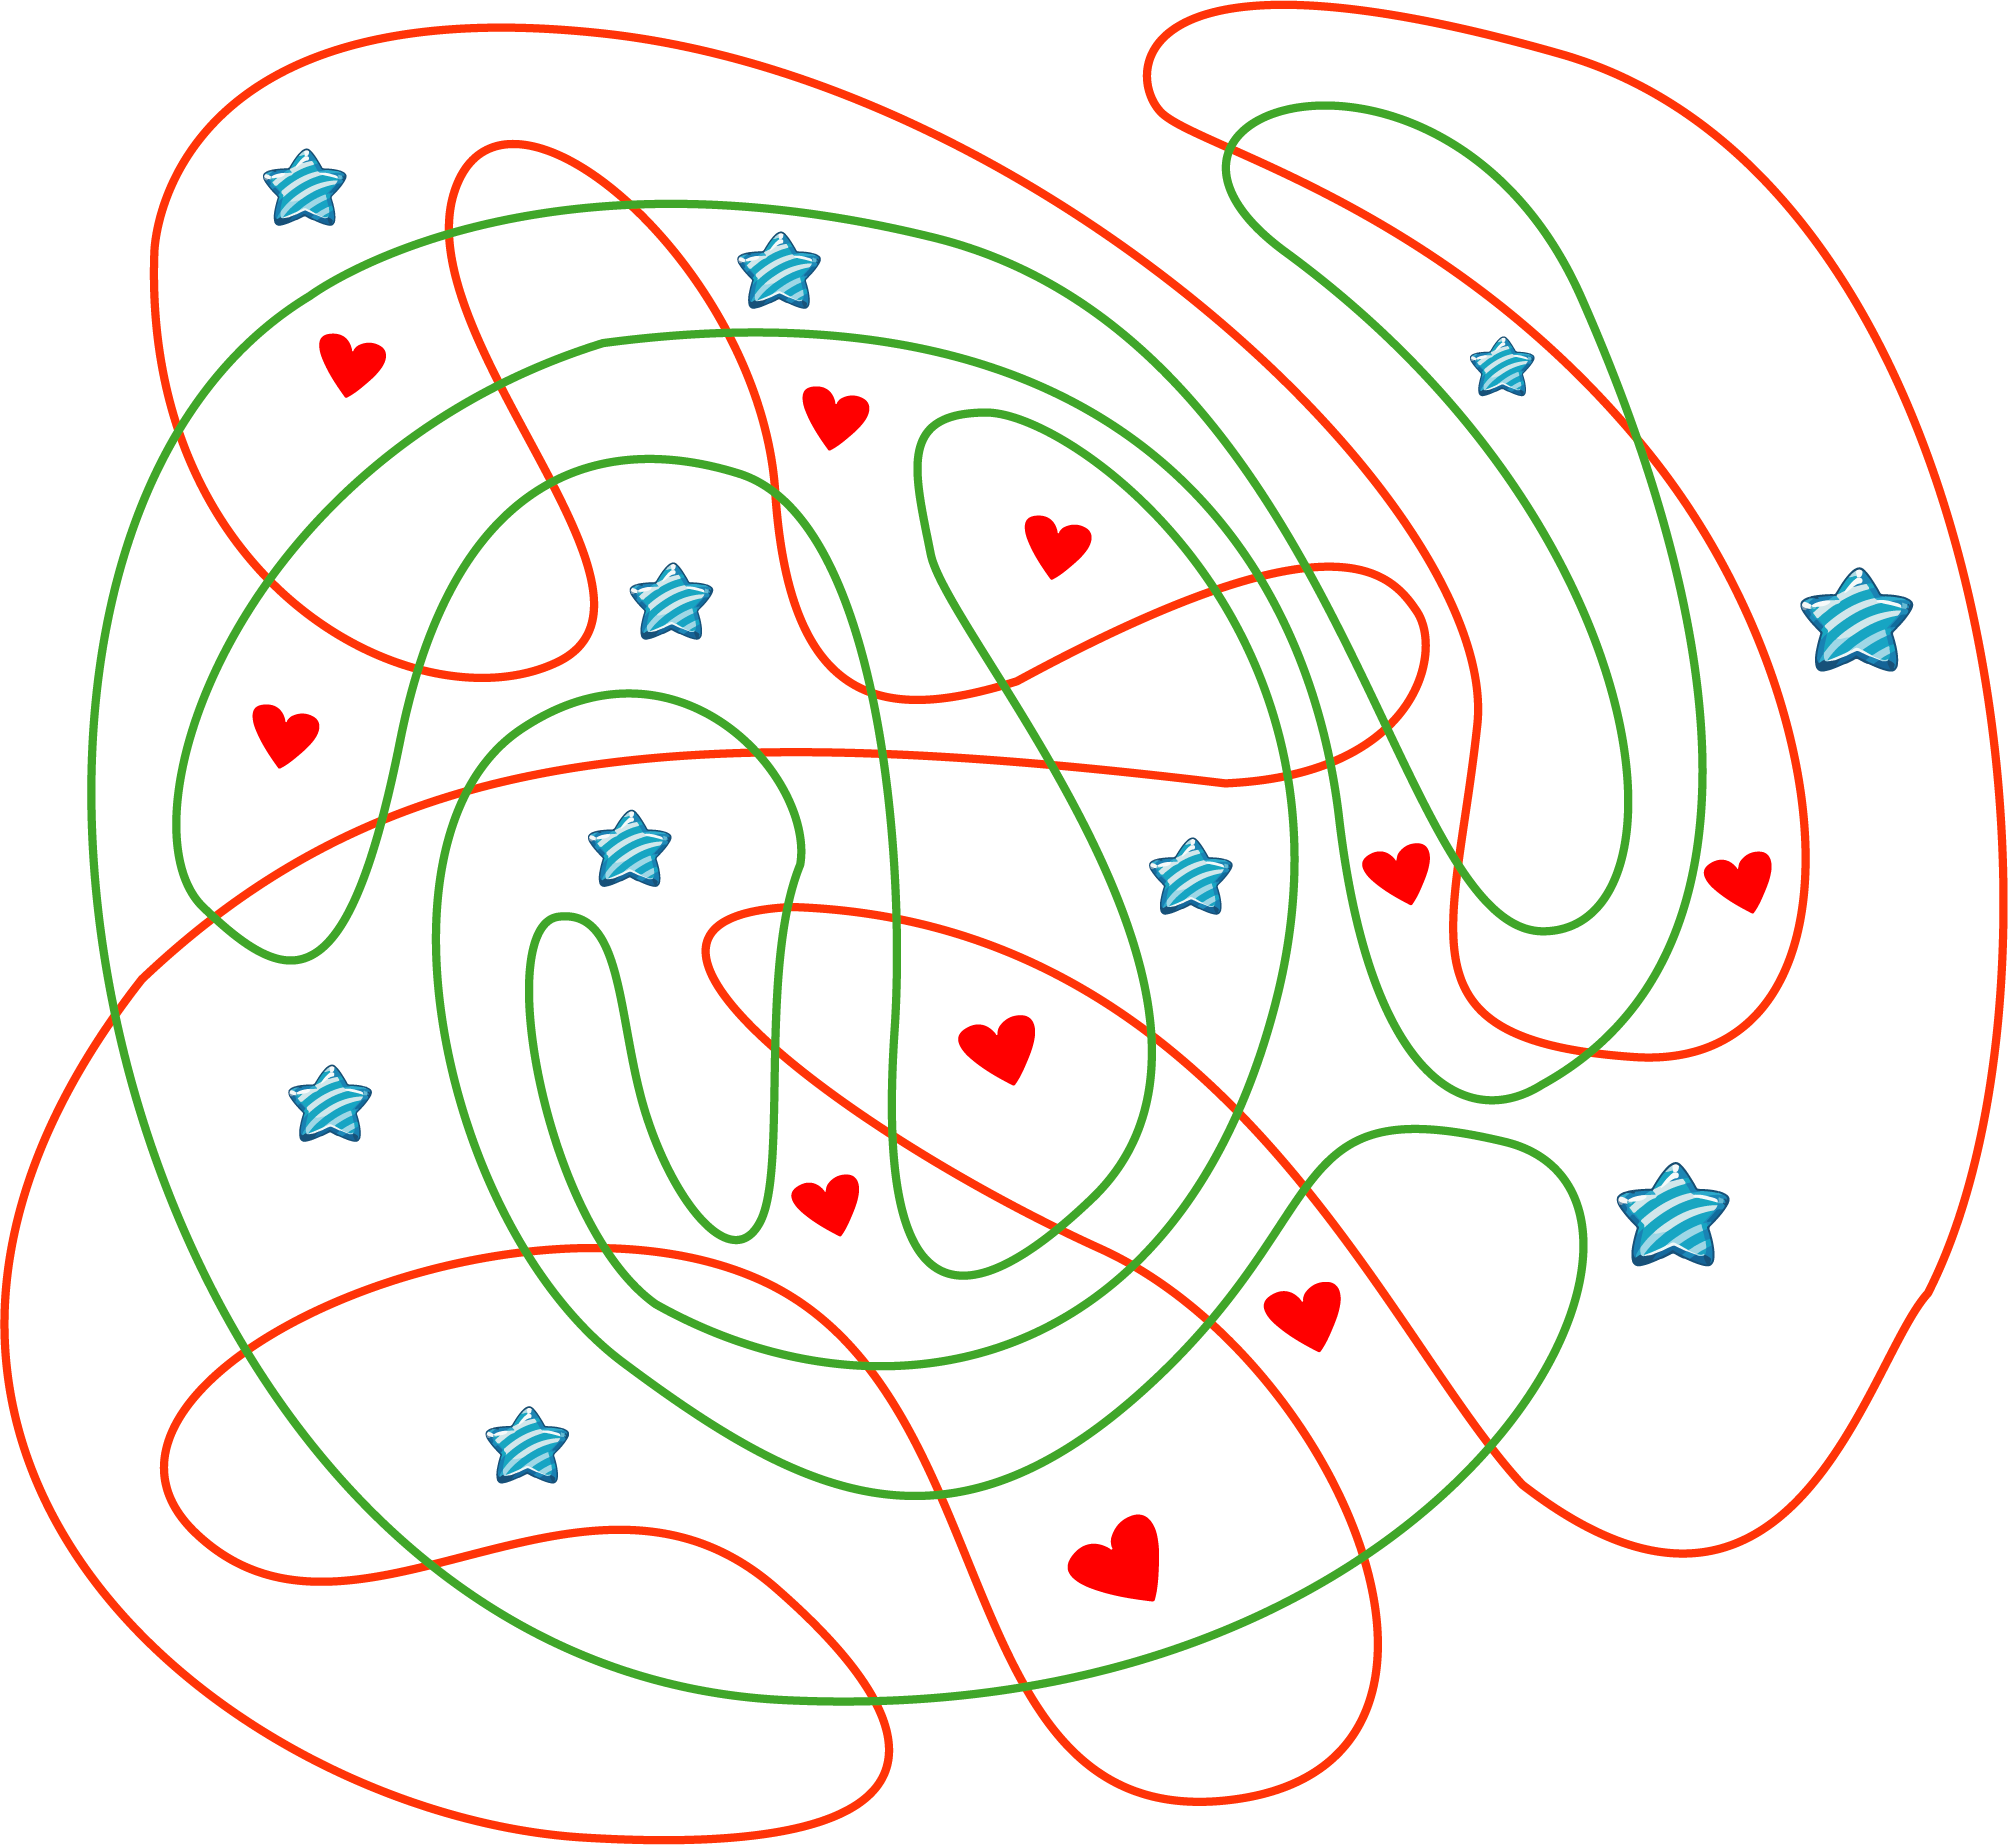
\includegraphics[width=0.38\textwidth]{8}
		\caption{\small\textit{Hình $8.$}}
		\vspace*{-10pt}
	\end{figure}
